\documentclass[12pt, letterpaper]{../assignment}
\usepackage{graphicx}
\usepackage{courier}
\usepackage{minted}
\usepackage{amsmath}
\usepackage{polynom}
\usepackage{commath}
\usepackage{amssymb}
\usepackage{amsfonts} 
\usepackage{color}
\usepackage{cancel}
\usepackage{enumitem}
\usepackage{graphicx}
\usepackage{multirow}
\usepackage{float}
\usepackage{bm}
\usepackage{tikz}
\usetikzlibrary{shapes,arrows}
\usepackage{booktabs}
\usetikzlibrary{patterns}

% Define Theme Colors
\definecolor{light-gray}{rgb}{0.2,0.2,0.2}
\definecolor{header-blue}{rgb}{0,0,0.7}
% \definecolor{header-blue}{rgb}{0.5137,0.8353,0.9176}
\definecolor{header-blue}{rgb}{0,0.8,0.95}
\definecolor{dark-gray}{rgb}{0.1,0.1,0.1}
\pagecolor{dark-gray}
\color{white}

\usemintedstyle{monokai}
\oddsidemargin = 0pt
\exercisesheet{Module 8}{Midterm Exam}
\student{Austin Barrilleaux}
\university{\color{header-blue}Johns Hopkins University}
\school{\color{header-blue}Whiting School of Engineering}
\courselabel{EN 535.612}
\semester{Fall 2024}
\usepackage[backend=bibtex,style=numeric,sorting=none]{biblatex}
\bibliography{reference}

\definecolor{light-gray}{rgb}{0.2,0.2,0.2}
\setminted{bgcolor=light-gray,frame=lines,rulecolor=white}
\setlength{\parindent}{0pt}

\makeatletter
\patchcmd{\minted@colorbg}{\noindent}{\medskip\noindent}{}{}
\apptocmd{\endminted@colorbg}{\par\medskip}{}{}
\makeatother


\begin{document}

\subsection*{Problem 1}
\subsubsection*{A satellite is in an orbit about the Earth.
The magnitude of the acceleration of this body is $\bm{g(R_e/R)^2}$,
where $\bm{R}$ is the distance from the body to  the center of the Earth,
$\bm{R_e = 6370}$ km is the radius of the Earth,
and $\bm{g = 9.807}\ \textbf{m}/\textbf{s}^2$.
At the position shown, the speed of the body is $\bm{v = 27\ 000 \textbf{km}/\textbf{h}}$.\\
(a) Determine the rate of change of the speed and the radius of curvature of the orbit at this position.\\
(b) Determine $\bm{\dot{R}}$, $\bm{\ddot{R}}$, $\bm{\dot{\theta}}$, and $\bm{\ddot{\theta}}$ at this position.}

\begin{figure}[H]
    \centering
    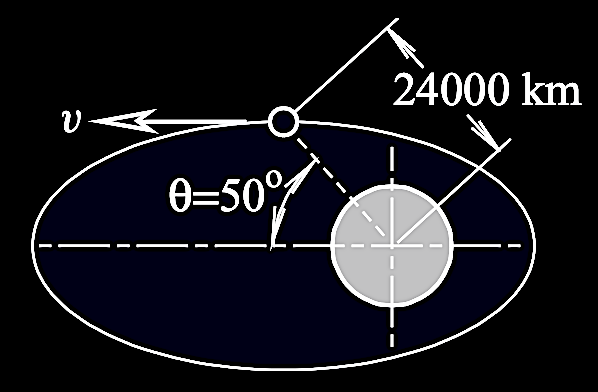
\includegraphics[scale=0.55,frame]{images/Problem_1.png}
\end{figure}

Sketching the following block diagram where, by inspection,
the unit tangent vector $e_t$ is parallel with the velocity vector,
and the normal direction unit vector $e_n$ extends toward the center of curvature
(which is toward the center of the elliptical orbit.)


\begin{center}

    \tikzset{every picture/.style={line width=0.75pt}} %set default line width to 0.75pt        

    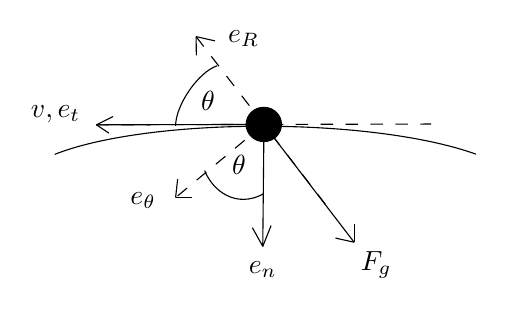
\begin{tikzpicture}[x=0.75pt,y=0.75pt,yscale=-1,xscale=1]
    %uncomment if require: \path (0,235); %set diagram left start at 0, and has height of 235
    
    %Shape: Arc [id:dp5609708917361678] 
    \draw  [draw opacity=0] (78.78,70.17) .. controls (99.75,61.78) and (138.28,56.32) .. (182.31,56.63) .. controls (223.72,56.92) and (260.21,62.24) .. (281.74,70.1) -- (182.11,85.65) -- cycle ; \draw   (78.78,70.17) .. controls (99.75,61.78) and (138.28,56.32) .. (182.31,56.63) .. controls (223.72,56.92) and (260.21,62.24) .. (281.74,70.1) ;  
    %Straight Lines [id:da5753428027341958] 
    \draw    (98.88,55.94) -- (179.5,55.75) ;
    %Flowchart: Connector [id:dp6687027633584581] 
    \draw  [fill={rgb, 255:red, 0; green, 0; blue, 0 }  ,fill opacity=1 ] (171,55.75) .. controls (171,51.19) and (174.81,47.5) .. (179.5,47.5) .. controls (184.19,47.5) and (188,51.19) .. (188,55.75) .. controls (188,60.31) and (184.19,64) .. (179.5,64) .. controls (174.81,64) and (171,60.31) .. (171,55.75) -- cycle ;
    %Straight Lines [id:da46457095104622814] 
    \draw    (179,114.5) -- (179.5,64) ;
    %Straight Lines [id:da07390647343570356] 
    \draw    (223,112.5) -- (179.5,55.75) ;
    %Straight Lines [id:da7232134312062481] 
    \draw  [dash pattern={on 4.5pt off 4.5pt}]  (146.88,13.44) -- (212.13,98.06) ;
    %Straight Lines [id:da15646105402572963] 
    \draw    (98.88,55.94) -- (106.88,51.94) ;
    %Straight Lines [id:da09244139347199365] 
    \draw    (104.88,59.94) -- (98.88,55.94) ;
    %Straight Lines [id:da006527953719763557] 
    \draw    (174,105.5) -- (179,114.5) ;
    %Straight Lines [id:da504994600380142] 
    \draw    (179,114.5) -- (183,104.5) ;
    %Straight Lines [id:da019968065751189146] 
    \draw    (214,110.5) -- (223,112.5) ;
    %Straight Lines [id:da7293082455780622] 
    \draw    (223,103.5) -- (223,112.5) ;
    %Curve Lines [id:da5442907492375646] 
    \draw    (137,56.5) .. controls (137,46.38) and (148,30.5) .. (157,27.5) ;
    %Straight Lines [id:da9878841341299782] 
    \draw    (147,22.5) -- (146.88,13.44) ;
    %Straight Lines [id:da49273640195015456] 
    \draw    (156,15.5) -- (146.88,13.44) ;
    %Straight Lines [id:da8219412910683288] 
    \draw  [dash pattern={on 4.5pt off 4.5pt}]  (98.88,55.94) -- (260.13,55.56) ;
    %Straight Lines [id:da6180368985701121] 
    \draw  [dash pattern={on 4.5pt off 4.5pt}]  (179.5,55.75) -- (137,91) ;
    %Straight Lines [id:da7552791067737405] 
    \draw    (137,91) -- (138,82) ;
    %Straight Lines [id:da9150337620515048] 
    \draw    (145,91) -- (137,91) ;
    %Curve Lines [id:da7268486900699349] 
    \draw    (179.25,89.25) .. controls (166.25,96.25) and (155,88) .. (151,78) ;
    
    % Text Node
    \draw (66,45.4) node [anchor=north west][inner sep=0.75pt]    {$v,e_{t}$};
    % Text Node
    \draw (171,120.4) node [anchor=north west][inner sep=0.75pt]    {$e_{n}$};
    % Text Node
    \draw (225,115.9) node [anchor=north west][inner sep=0.75pt]    {$F_{g}$};
    % Text Node
    \draw (148,38.4) node [anchor=north west][inner sep=0.75pt]    {$\theta $};
    % Text Node
    \draw (161,9.4) node [anchor=north west][inner sep=0.75pt]    {$e_{R}$};
    % Text Node
    \draw (163,69.4) node [anchor=north west][inner sep=0.75pt]    {$\theta $};
    % Text Node
    \draw (114,87.4) node [anchor=north west][inner sep=0.75pt]    {$e_{\theta }$};
    
    
    \end{tikzpicture}
    
\end{center}

From this, we can define the unit tangent vector as: %and the normal direction unit vector as:

$$ \bar{e}_t = \left[\begin{array}{rr} \cos\left(\theta \right) & -\sin\left(\theta \right)\\ \sin\left(\theta \right) & \cos\left(\theta \right) \end{array}\right]
\left[\begin{array}{rr} 1\\ 0 \end{array}\right] = 
\left[\begin{array}{c} \cos\left(\theta \right) \ \bar{e}_R \\ \sin\left(\theta \right) \ \bar{e}_\theta \end{array}\right]  $$

Because $\dot{v}$ is the tangential component of acceleration, we find that:

$$ \dot{v} = \bar{a} \cdot \bar{e}_t = g\left(\frac{R_e}{R}\right)^2
\left[\begin{array}{rr} -1 \ \bar{e}_R \\ 0 \ \bar{e}_\theta \end{array}\right]\cdot
\left[\begin{array}{c} \cos\left(\theta \right) \ \bar{e}_R \\ \sin\left(\theta \right) \ \bar{e}_\theta \end{array}\right]
= -9.807\left(\frac{6370 \times 10^3}{24000 \times 10^3}\right)^2 \cos\left(\theta \right)  $$

This evaluates to:

\begin{answer}
$$ \dot{v} = -0.4441 \ \textbf{m}/\textbf{s}^2  $$
\end{answer}

Looking at the equation for acceleration:

$$ \bar{a} = \dot{v} \bar{e}_t + \frac{v^2}{\rho}\bar{e}_n $$

To solve for the radius of curvature:

$$ \frac{v^2}{\rho}\bar{e}_n = \bar{a} -\dot{v} \bar{e}_t \ \rightarrow
\ \rho = \frac{v^2}{|\bar{a} -\dot{v} \bar{e}_t|} $$

The radius of curvature is:

$$ \rho = \frac{v^2}{|\bar{a} -\dot{v} \bar{e}_t|} =
\frac{\left(27\ 000 \times 10^3/3600\right)^2}{\left|-9.807\left(\frac{6370 \times 10^3}{24000 \times 10^3}\right)^2
\left[\begin{array}{rr} -1\ \bar{e}_R\\ 0 \ \bar{e}_\theta \end{array}\right] -\left(-0.4441\right) 
\left[\begin{array}{c} \cos\left(\theta \right) \ \bar{e}_R \\ \sin\left(\theta \right)\ \bar{e}_\theta \end{array}\right]\right|}
$$

This evaluates to:

\begin{answer}
$$ \rho = 1.0629 \times 10^8 \ \textbf{m}  $$
\end{answer}


Using the following velocity equation:

$$ \bar{v} = \dot{R}\ \bar{e}_R + R \dot{\theta}\ \bar{e}_\theta $$

Looking at the sketch:

$$ \bar{v} = \left(\frac{27\ 000 \times 10^3}{3600}\right)
\left[\begin{array}{c} \cos\left(\theta \right) \ \bar{e}_R \\ \sin\left(\theta \right)\ \bar{e}_\theta \end{array}\right]$$

From these two equations we get that:

\begin{answer}
\begin{equation*}
    \begin{aligned}
        \dot{R} &= \left(\frac{27\ 000 \times 10^3}{3600}\right)\cos\left(\theta \right)
        = 4820.9  \ \textbf{m}/\textbf{s}\\
        \dot{\theta}& = \left(\frac{27\ 000 \times 10^3}{3600}\right)\sin\left(\theta \right)/R
        = 0.0002393  \ \textbf{rad}/\textbf{s}
    \end{aligned}
\end{equation*}
\end{answer}

Using the following acceleration equation:

$$ \bar{a} = \left( \ddot{R} - R \dot{\theta}^2 \right)\bar{e}_R +
\left( R\ddot{\theta} + 2\dot{R}\dot{\theta} \right)\bar{e}_\theta$$

Where:

$$ \bar{a} = -9.807\left(\frac{6370 \times 10^3}{24000 \times 10^3}\right)^2
\left[\begin{array}{rr} -1\ \bar{e}_R\\ 0 \ \bar{e}_\theta \end{array}\right] $$

We get that:

\begin{answer}
\begin{equation*}
    \begin{aligned}
        \ddot{R} &= \bar{a} \cdot \bar{e}_R + R \dot{\theta}^2
        = 0.6845  \ \textbf{m}/\textbf{s}^2\\
        \ddot{\theta}& = \left( \cancelto{0}{\bar{a} \cdot \bar{e}_\theta} - 2\dot{R}\dot{\theta} \right)/R = 
        -9.617\times 10^8 \ \textbf{rad}/\textbf{s}^2
    \end{aligned}
\end{equation*}
\end{answer}

The following MATLAB script was used to solve this problem:
% \color{white}
\hspace*{6em}\inputminted[frame=leftline,fontsize=\footnotesize]{matlab}
{./matlab/Problem_1.m}
% \color{black} 

\subsection*{Problem 2}
\subsubsection*{The disk spins about its axis C D at 1200 rev/min as the system rotates about the vertical axis at 20 rev/min.
Both rates are constant.
The angle of elevation of the arm supporting the disk is such that $\bm{\dot{\beta} = 10}$ rad/s and $\bm{\ddot{\beta} = -500}\ \textbf{rad/s}^2$  when $\bm{\beta = 36.87^\circ}$.
Determine the velocity and acceleration of point E,
which is the lowest point on the perimeter of the disk.
Note: the solution for velocity in the text is for a clockwise rotation about the vertical axis}

\begin{figure}[H]
    \centering
    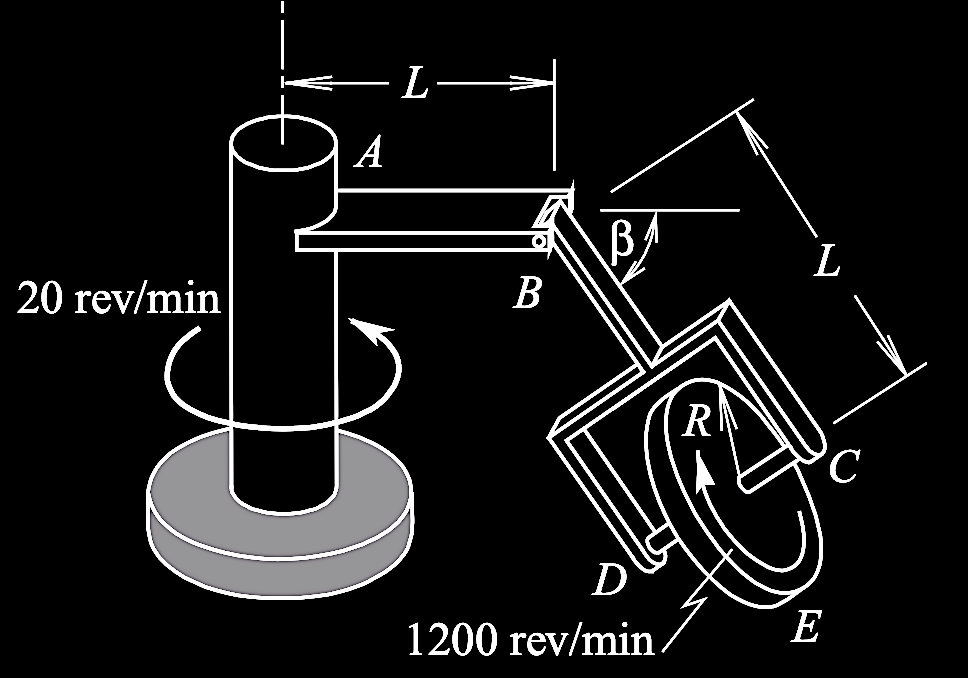
\includegraphics[scale=0.5,frame]{images/Problem_2.png}
\end{figure}

We will solve this problem consistent with the note in the prompt.
\\\\
We will define the following coordinate frames for the system:

\begin{centering}


    \tikzset{every picture/.style={line width=0.75pt}} %set default line width to 0.75pt        

    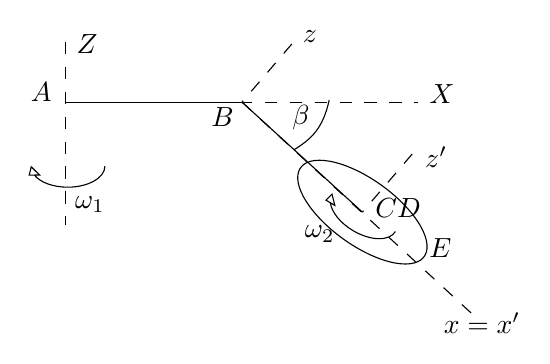
\begin{tikzpicture}[x=0.75pt,y=0.75pt,yscale=-1,xscale=1]
    %uncomment if require: \path (0,182); %set diagram left start at 0, and has height of 182
    
    %Straight Lines [id:da30022602593809844] 
    \draw    (62,54) -- (147,54) ;
    %Straight Lines [id:da8288788542415915] 
    \draw    (147,54) -- (205,107) ;
    %Flowchart: Connector [id:dp18393682558043611] 
    \draw   (181.71,107) .. controls (170.27,93.19) and (171.43,82) .. (184.29,82) .. controls (197.15,82) and (216.85,93.19) .. (228.29,107) .. controls (239.73,120.81) and (238.57,132) .. (225.71,132) .. controls (212.85,132) and (193.15,120.81) .. (181.71,107) -- cycle ;
    %Straight Lines [id:da08328645583785521] 
    \draw  [dash pattern={on 4.5pt off 4.5pt}]  (62,54) -- (232,54) ;
    %Curve Lines [id:da0493598542143765] 
    \draw    (189,53) .. controls (186,67) and (180,72) .. (172,77) ;
    %Straight Lines [id:da10927227437478448] 
    \draw  [dash pattern={on 4.5pt off 4.5pt}]  (62,25) -- (62,113) ;
    %Straight Lines [id:da9966612794201675] 
    \draw  [dash pattern={on 4.5pt off 4.5pt}]  (171,26) -- (147,54) ;
    %Straight Lines [id:da14869123950977747] 
    \draw  [dash pattern={on 4.5pt off 4.5pt}]  (147,54) -- (260,158) ;
    %Straight Lines [id:da3432297912367157] 
    \draw  [dash pattern={on 4.5pt off 4.5pt}]  (229,79) -- (205,107) ;
    %Curve Right Arrow [id:dp22372090927053256] 
    \draw  [fill={rgb, 255:red, 255; green, 255; blue, 255 }  ,fill opacity=1 ] (63.3,94.99) .. controls (73.1,94.9) and (81,90.35) .. (80.95,84.82) -- (80.95,84.82) .. controls (81,90.35) and (73.1,94.9) .. (63.3,94.99) -- cycle ;\draw  [fill={rgb, 255:red, 255; green, 255; blue, 255 }  ,fill opacity=1 ] (63.3,94.99) .. controls (56.02,95.06) and (49.74,92.65) .. (46.97,89.14) -- (49.47,89.12) -- (45.45,85.15) -- (44.47,89.16) -- (46.97,89.14) .. controls (49.74,92.65) and (56.02,95.06) .. (63.3,94.99) -- cycle ;
    %Curve Right Arrow [id:dp9745312713561716] 
    \draw  [fill={rgb, 255:red, 255; green, 255; blue, 255 }  ,fill opacity=1 ] (200.53,115.94) .. controls (208.97,120.93) and (218.09,121.11) .. (220.9,116.36) -- (220.9,116.36) .. controls (218.09,121.11) and (208.97,120.93) .. (200.53,115.94) -- cycle ;\draw  [fill={rgb, 255:red, 255; green, 255; blue, 255 }  ,fill opacity=1 ] (200.53,115.94) .. controls (194.27,112.24) and (190.14,106.93) .. (189.57,102.5) -- (191.73,103.77) -- (190.34,98.3) -- (187.42,101.23) -- (189.57,102.5) .. controls (190.14,106.93) and (194.27,112.24) .. (200.53,115.94) -- cycle ;
    
    % Text Node
    \draw (170,54.4) node [anchor=north west][inner sep=0.75pt]    {$\beta $};
    % Text Node
    \draw (66,20.4) node [anchor=north west][inner sep=0.75pt]    {$Z$};
    % Text Node
    \draw (175,18.4) node [anchor=north west][inner sep=0.75pt]    {$z$};
    % Text Node
    \draw (234,74.4) node [anchor=north west][inner sep=0.75pt]    {$z'$};
    % Text Node
    \draw (243,154.4) node [anchor=north west][inner sep=0.75pt]    {$x=x'$};
    % Text Node
    \draw (236,44.4) node [anchor=north west][inner sep=0.75pt]    {$X$};
    % Text Node
    \draw (65.3,98.39) node [anchor=north west][inner sep=0.75pt]    {$\omega _{1}$};
    % Text Node
    \draw (176,112.4) node [anchor=north west][inner sep=0.75pt]    {$\omega _{2}$};
    % Text Node
    \draw (44,43.4) node [anchor=north west][inner sep=0.75pt]    {$A$};
    % Text Node
    \draw (131,55.4) node [anchor=north west][inner sep=0.75pt]    {$B$};
    % Text Node
    \draw (210,99.4) node [anchor=north west][inner sep=0.75pt]    {$CD$};
    % Text Node
    \draw (236,118.4) node [anchor=north west][inner sep=0.75pt]    {$E$};
    
    
    \end{tikzpicture}
    
\end{centering}

You will note that the \{xyz\} frame and \{x'y'z'\} frame are identical for this problem,
so I will use \{xyz\} to express the coordinate frame at both points from this point.

Constructing the angular velocity vector $\bar{\omega}$ of $\left\{xyz\right\}$ by vectorially adding the simple rotation rates according to:

$$ \bar{\omega} = \omega_1 \bar{e}_1 + \omega_2 \bar{e}_2  + \omega_3 \bar{e}_3$$

This gives us:

$$ \bar{\omega} = -\omega_1 K+ \dot{\beta} j - \omega_2 k$$

Using the following coordinate transformation:

$$ R_\text{rot} = 
\left[\begin{array}{ccc} \cos\left(\beta \right) & 0 & -\sin\left(\beta \right)\\ 0 & 1 & 0\\ \sin\left(\beta \right) & 0 & \cos\left(\beta \right) \end{array}\right]
$$

$$ K = R_\text{rot}
\left[\begin{array}{ccc} 0 \ I \\ 0 \ J \\1 \ K \end{array}\right] = 
\left[\begin{array}{r} -\sin\left(\beta \right) \ i\\ 0 \ j\\ \cos\left(\beta \right) \ k \end{array}\right]
= -\sin\left(\beta \right) i + \cos\left(\beta \right) k$$

This gives us the angular velocity vector in the form:

$$ \bar{\omega} = \left[\begin{array}{r} \omega _{1}\,\sin\left(\beta \right) \ i \\ \dot{\beta } \ j \\ -\omega _{2}-\omega _{1}\,\cos\left(\beta \right) \ k  \end{array}\right] $$

For the angular rotations, the angular velocity is:

\begin{equation*}
\begin{aligned}
\Omega_1 &= -\omega_1 K= \left[\begin{array}{r} \omega _{1}\,\sin\left(\beta \right) \ i \\ 0 \ j \\ -\omega _{1}\,\cos\left(\beta \right) \ k  \end{array}\right]\\
\Omega_2 &= -\omega_1 K+ \dot{\beta} j = \left[\begin{array}{r} \omega _{1}\,\sin\left(\beta \right) \ i \\ \dot{\beta } \ j \\ -\omega _{1}\,\cos\left(\beta \right) \ k  \end{array}\right]\\
\Omega_3 &= \bar{\omega}
\end{aligned}
\end{equation*}

Using the following relative positions:

\begin{equation*}
    \begin{aligned}
        \bar{r}_{B/A} &= L\left(\begin{array}{c} \cos\left(\beta \right)\ i\\ 0 \ j\\ \sin\left(\beta \right) \ k \end{array}\right)\\
        \bar{r}_{CD/B} &= L\ i\\
        \bar{r}_{E/CD} &= R\ i\\
    \end{aligned}
\end{equation*}

Referencing the velocity equation:

$$ \bar{v}_P = \bar{v}_O + \bar{\omega} \times \bar{r}_{P/O}$$
    
We solve for the velocities along the system from A to E:

\begin{equation*}
    \begin{aligned}
        \bar{v}_B &= \Omega_1 \times \bar{r}_{B/A} = \left[\begin{array}{c} 0\\ -2.0944\,L\\ 0 \end{array}\right] \\
        \bar{v}_{CD} &= \bar{v}_B + \Omega_2 \times \bar{r}_{CD/B} = \left[\begin{array}{c} 0\\ -3.7699\,L\\ -10\,L \end{array}\right] \\
        \bar{v}_E &= \bar{v}_{CD} + \Omega_3 \times \bar{r}_{E/CD} = \left[\begin{array}{c} 0\\ -3.7699\,L-127.34\,R\\ -10\,L-10\,R \end{array}\right]
    \end{aligned}
\end{equation*}

Therefore:

\begin{answer}
$$ \bar{v}_E =   -\left(3.7699\,L+127.34\,R\right) j - 10\left(L+R \right)k $$
\end{answer}

We can solve for the angular rotation at the rotation points using the equation for angular acceleration:

$$ \bar{\alpha} =
\sum_n \left( \dot{\omega}_n \bar{e}_n + \bar{\Omega}_n \times \omega_n \bar{e}_n \right) $$

The relative angular accelerations across the system for points A to E are:

\begin{equation*}
\begin{aligned}
\bar{\alpha}_1 &= \Omega_1 \times \Omega_1 = 0\\
\bar{\alpha}_2 &= \bar{\alpha}_1 + \ddot{\beta} j + \Omega_2 \times \dot{\beta} j\\
\bar{\alpha}_3 &= \bar{\alpha}_2 + \Omega_3 \times \omega_2(-k) = \bar{\alpha} % alpha_bar
\end{aligned}
\end{equation*}

Using the acceleration equation:

$$ \bar{a}_P = \bar{a}_O + \bar{\alpha} \times \bar{r}_{P/O} + \bar{\omega} \times \left( \bar{\omega} \times \bar{r}_{P/O} \right)$$

Solving for the acceleration across the system for points A to E:

\begin{equation*}
    \begin{aligned}
        \bar{a}_B &= 0 + \bar{\alpha}_1 \times \bar{r}_{B/A} + \Omega_1 \times \left(\Omega_1 \times \bar{r}_{B/A}\right)
        =\left[\begin{array}{c} -3.5092\,L\\ 0\\ -2.6319\,L \end{array}\right]\\
        \bar{a}_{CD} &= \bar{a}_B + \bar{\alpha}_2 \times \bar{r}_{CD/B} + \Omega_2 \times \left(\Omega_2 \times \bar{r}_{CD/B}\right)
        =\left[\begin{array}{c} -106.32\,L\\ 25.133\,L\\ 495.26\,L \end{array}\right]\\
        \bar{a}_E &= \bar{a}_{CD} + \bar{\alpha}_3 \times \bar{r}_{E/CD} + \Omega_3 \times \left(\Omega_3 \times \bar{r}_{E/CD}\right)
        =\left[\begin{array}{c} -106.32\,L-16315\,R\\ 25.133\,L+25.133\,R\\ 495.26\,L+182.07\,R \end{array}\right]
    \end{aligned}
\end{equation*}

Therefore:

\begin{answer}
$$ a_E = -(106.32\,L+16315\,R)\ i + 25.133(L+R)\ j + (495.26\,L+182.07\,R)\ k $$
\end{answer}


If I solve this for the solution where the vertical axis rotation is counter clockwise,
we get that:

\begin{answer}
    \begin{equation*}
        \begin{aligned}
    v_E &= \left( 0.4189L - 127.3392R \right)j - 10 \left(L+R\right)k \\
    a_E &= -(106.32\,L+16315\,R)\ i + 25.133(L+R)\ j + (495.26\,L+182.07\,R)\ k 
\end{aligned}
\end{equation*}
\end{answer}
    

These solutions match the text.
\\\\
The following MATLAB script was used to solve this problem:
% \color{white}
\hspace*{6em}\inputminted[frame=leftline,fontsize=\footnotesize]{matlab}
{./matlab/Problem_2.m}
% \color{black} 

\subsection*{Problem 3}
\subsubsection*{The gyroscopic turn indicator consists of a 1-kg flywheel whose principal radii of gyration are $\bm{k =50}$ mm and $\bm{k = k = 40}$ mm.
The center of mass of the flywheel coincides with the intersection of axes AB and CD.
The flywheel spins relative to the gimbal at the constant rate $\bm{\omega_1 = 10,000}$ rev/min.
A couple $\bm{\bar{M}}$ acts about shaft CD,
which supports the gimbal,
in order to control the angle $\bm{\beta}$  between the gimbal and the horizontal.
Determine $\bm{\bar{M}}$ when the rotation rate about the vertical axis is $\bm{\Omega = 0.8}$ rad/s.}

\begin{figure}[H]
    \centering
    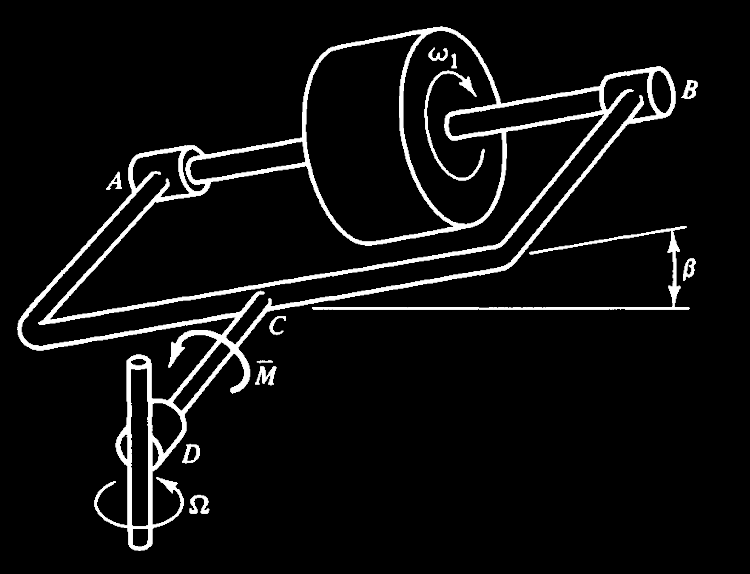
\includegraphics[scale=0.5,frame]{images/Problem_3.png}
\end{figure}

We will define the following frames for the system:

\begin{center}

    \tikzset{every picture/.style={line width=0.75pt}} %set default line width to 0.75pt        

    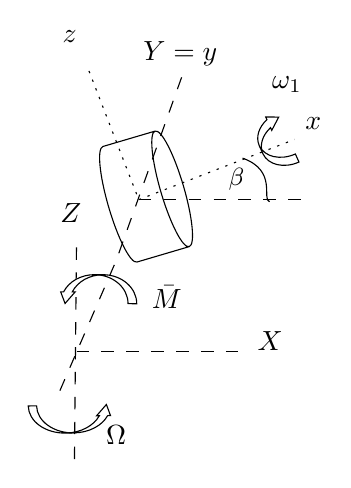
\begin{tikzpicture}[x=0.75pt,y=0.75pt,yscale=-1,xscale=1]
    %uncomment if require: \path (0,235); %set diagram left start at 0, and has height of 235
    
    %Straight Lines [id:da0462652485240338] 
    \draw  [dash pattern={on 4.5pt off 4.5pt}]  (98,182) -- (125.15,119.23) -- (157,30) ;
    %Straight Lines [id:da2781887940807206] 
    \draw  [dash pattern={on 4.5pt off 4.5pt}]  (136,90) -- (219,90) ;
    %Straight Lines [id:da0781192111029887] 
    \draw  [dash pattern={on 0.84pt off 2.51pt}]  (136,90) -- (211,61) ;
    %Straight Lines [id:da6711962405398284] 
    \draw  [dash pattern={on 0.84pt off 2.51pt}]  (112,28) -- (136,90) ;
    %Curve Lines [id:da9209612993523657] 
    \draw    (186,70) .. controls (203,76) and (195,90) .. (199,91) ;
    %Curve Right Arrow [id:dp14539415705721326] 
    \draw  [fill={rgb, 255:red, 255; green, 255; blue, 255 }  ,fill opacity=1 ] (104.84,202.37) .. controls (94.99,202.57) and (86.9,196.72) .. (86.75,189.32) -- (82.73,189.4) .. controls (82.88,196.8) and (90.97,202.65) .. (100.82,202.45) ;\draw  [fill={rgb, 255:red, 255; green, 255; blue, 255 }  ,fill opacity=1 ] (100.82,202.45) .. controls (108.13,202.31) and (114.34,198.88) .. (117,194.09) -- (115.66,194.12) -- (120.39,188.67) -- (122.36,193.99) -- (121.02,194.02) .. controls (118.36,198.8) and (112.15,202.23) .. (104.84,202.37)(100.82,202.45) -- (104.84,202.37) ;
    %Shape: Can [id:dp3314145556815138] 
    \draw   (160.27,112.63) -- (135.14,120.04) .. controls (132.16,120.92) and (126.08,109.16) .. (121.55,93.79) .. controls (117.02,78.42) and (115.75,65.24) .. (118.73,64.37) -- (143.86,56.96) .. controls (146.84,56.08) and (152.92,67.84) .. (157.45,83.21) .. controls (161.98,98.58) and (163.25,111.76) .. (160.27,112.63) .. controls (157.3,113.51) and (151.21,101.76) .. (146.68,86.38) .. controls (142.15,71.01) and (140.89,57.84) .. (143.86,56.96) ;
    %Straight Lines [id:da31109279394214395] 
    \draw  [dash pattern={on 4.5pt off 4.5pt}]  (106,163) -- (189,163) ;
    %Straight Lines [id:da8479867066098676] 
    \draw  [dash pattern={on 4.5pt off 4.5pt}]  (105,215) -- (106,111) ;
    %Curve Right Arrow [id:dp15885928167198493] 
    \draw  [fill={rgb, 255:red, 255; green, 255; blue, 255 }  ,fill opacity=1 ] (194.04,63.97) .. controls (196.49,69.41) and (204.28,71.21) .. (211.43,67.98) -- (213.18,71.87) .. controls (206.03,75.09) and (198.24,73.29) .. (195.79,67.85) ;\draw  [fill={rgb, 255:red, 255; green, 255; blue, 255 }  ,fill opacity=1 ] (195.79,67.85) .. controls (193.97,63.81) and (195.59,58.89) .. (199.48,55.31) -- (200.06,56.61) -- (203.41,50.22) -- (197.14,50.14) -- (197.73,51.43) .. controls (193.84,55.01) and (192.21,59.93) .. (194.04,63.97)(195.79,67.85) -- (194.04,63.97) ;
    %Curve Right Arrow [id:dp7167518498909757] 
    \draw  [fill={rgb, 255:red, 255; green, 255; blue, 255 }  ,fill opacity=1 ] (114.65,126.13) .. controls (123.61,126.16) and (130.84,132.42) .. (130.82,140.11) -- (135,140.13) .. controls (135.02,132.44) and (127.78,126.18) .. (118.83,126.15) ;\draw  [fill={rgb, 255:red, 255; green, 255; blue, 255 }  ,fill opacity=1 ] (118.83,126.15) .. controls (112.18,126.13) and (106.46,129.54) .. (103.94,134.45) -- (105.33,134.46) -- (100.48,140.01) -- (98.37,134.44) -- (99.76,134.44) .. controls (102.28,129.53) and (108,126.11) .. (114.65,126.13)(118.83,126.15) -- (114.65,126.13) ;
    
    % Text Node
    \draw (178,73.4) node [anchor=north west][inner sep=0.75pt]  [font=\small]  {$\beta $};
    % Text Node
    \draw (192,152.4) node [anchor=north west][inner sep=0.75pt]    {$X$};
    % Text Node
    \draw (98,7.4) node [anchor=north west][inner sep=0.75pt]    {$z$};
    % Text Node
    \draw (119,197.49) node [anchor=north west][inner sep=0.75pt]    {$\Omega$};
    % Text Node
    \draw (97,90.4) node [anchor=north west][inner sep=0.75pt]    {$Z$};
    % Text Node
    \draw (137,12.4) node [anchor=north west][inner sep=0.75pt]    {$Y=y$};
    % Text Node
    \draw (215,49.4) node [anchor=north west][inner sep=0.75pt]    {$x$};
    % Text Node
    \draw (199,29.4) node [anchor=north west][inner sep=0.75pt]    {$\omega _{1}$};
    % Text Node
    \draw (141,130.4) node [anchor=north west][inner sep=0.75pt]    {$\bar{M}$};
    
    
    \end{tikzpicture}

\end{center}

For this problem the prompt seems to imply that the rotation rate about the vertical axis is constant. 
\\\\
Constructing the angular velocity vector $\bar{\omega}$ of $\left\{xyz\right\}$ by vectorially adding the simple rotation rates according to:

$$ \bar{\omega} = \omega_1 \bar{e}_1 + \omega_2 \bar{e}_2 $$

This gives us:

$$ \bar{\omega} = \Omega K + \omega_1 (-i)$$

Using the following coordinate transformation:

$$ R_\text{rot} = 
\left[\begin{array}{ccc} \cos\left(-\beta \right) & 0 & -\sin\left(-\beta \right)\\ 0 & 1 & 0\\ \sin\left(-\beta \right) & 0 & \cos\left(-\beta \right) \end{array}\right]
$$

$$ K = R_\text{rot}
\left[\begin{array}{ccc} 0 \ I \\ 0 \ J \\1 \ K \end{array}\right] = 
\left[\begin{array}{c} \sin\left(\beta \right)\\ 0\\ \cos\left(\beta \right) \end{array}\right]
= \sin\left(\beta \right) i + \cos\left(\beta \right) k$$

This gives us the angular velocity vector in the form:

$$ \bar{\omega} = \left[\begin{array}{r} \left(\Omega \,\sin\left(\beta \right)-\omega _{1}\right)\ i \\ 0\ j \\ \Omega \,\cos\left(\beta \right) \ k \end{array}\right]
= \left(\Omega \,\sin\left(\beta \right)-\omega _{1}\right) i + \Omega \,\cos\left(\beta \right)k $$

Using the equation for angular acceleration:

$$ \bar{\alpha} =
\sum_n \left( \dot{\omega}_n \bar{e}_n + \bar{\Omega}_n \times \omega_n \bar{e}_n \right) $$

We see compute that the angular acceleration is:

$$ \bar{\alpha} = \bar{\omega} \times \omega_1 (-i) = 
-\Omega \,\omega _{1}\,\cos\left(\beta \right) j $$

Since the torque $\bar{M}$ is acting in the $j$ direction,
we can refer to equation 6.1.6 in the textbook:

$$ \sum \bar{M} \ j =  I_{yy}\alpha_y +
    \left( I_{zz} - I_{xx} \right) \omega_x \omega_z $$

Solving for the principal axis inertia quantities:

\begin{equation*}
    \begin{aligned}
        I_{xx} &= m k_1^2 = (1\ \text{kg})\left(\frac{50}{1000} \ \text{m} \right)^2 = 0.0025\ \text{kg-m}^2\\
        I_{yy} = I_{zz} &= m k_2^2 = (1\ \text{kg})\left(\frac{40}{1000} \ \text{m} \right)^2 = 0.0016\ \text{kg-m}^2
    \end{aligned}
\end{equation*}

We can solve for $\bar{M}$ as:

\begin{equation*}
\begin{aligned}
\bar{M} &=  0.0016 \left( -\Omega \,\omega _{1}\,\cos\left(\beta \right) \right) +
    \left( 0.0016 - 0.0025 \right) \left(\Omega \,\sin\left(\beta \right)-\omega _{1}\right)\left(\Omega \,\cos\left(\beta \right)\right) \\
    &=  0.0016 \left( -0.8\left(\frac{10000(2\pi)}{60}\right)\,\cos\left(\beta \right) \right) +\\
    & \ \ \ \ \ \ \ \ \ \left( 0.0016 - 0.0025 \right) \left(0.8 \,\sin\left(\beta \right)-\left(\frac{10000(2\pi)}{60}\right)\right)\left(0.8 \,\cos\left(\beta \right)\right)\\
    &= 0.000576 \cos(\beta)\sin(\beta) - 2.0944\cos(\beta)\ \text{N-m}
\end{aligned}
\end{equation*}

The couple $\bm{\bar{M}}$ when the rotation rate about the vertical axis is $\bm{\Omega = 0.8}$ rad/s is:

\begin{answer}
    \begin{equation*}
        \begin{aligned}
        \bar{M} &= 0.000576 \cos(\beta)\sin(\beta) - 2.0944\cos(\beta)\ \textbf{N-m}
        \end{aligned}
        \end{equation*}
\end{answer}

The following MATLAB script was used to solve this problem:
% \color{white}
\hspace*{6em}\inputminted[frame=leftline,fontsize=\footnotesize]{matlab}
{./matlab/Problem_3.m}
% \color{black} 

\subsection*{Problem 4}
\subsubsection*{A 50-kg rectangular plate is mounted diagonally on a shaft whose mass is negligible.
The system was initially at rest when a constant torque of 5 kN-m is applied to the shaft.
Determine the reactions at bearings A and B four seconds after the application of the torque.
}

\begin{figure}[H]
    \centering
    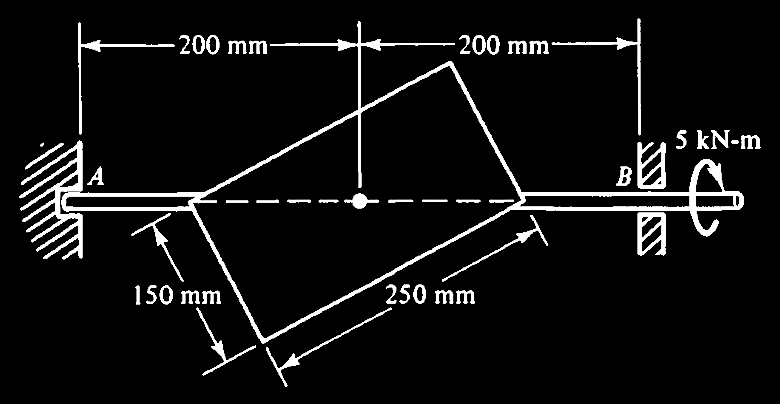
\includegraphics[scale=0.7,frame]{images/Problem_4.png}
\end{figure}

The following sketch details the body fixed frames $\left\{xyz\right\}$ and $\left\{x'y'z'\right\}$
and the reaction forces $F_A$ and $F_B$.

\begin{center}
    

\tikzset{every picture/.style={line width=0.75pt}} %set default line width to 0.75pt        

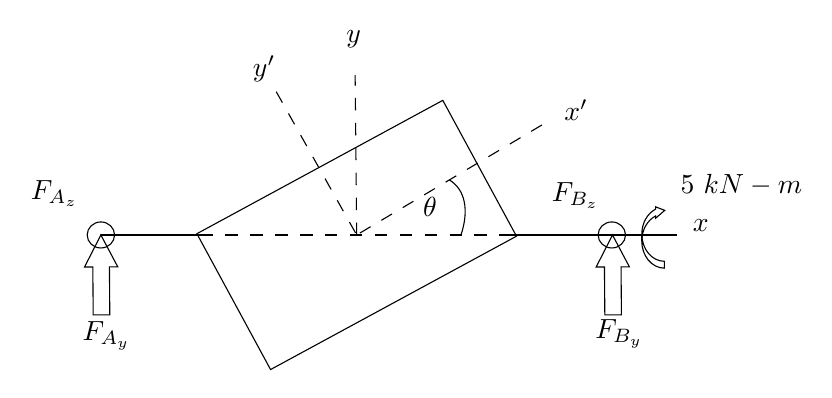
\begin{tikzpicture}[x=0.75pt,y=0.75pt,yscale=-1,xscale=1]
%uncomment if require: \path (0,235); %set diagram left start at 0, and has height of 235

%Flowchart: Process [id:dp1937554667130883] 
\draw   (152.26,116.4) -- (270.74,52.15) -- (306.24,117.6) -- (187.76,181.85) -- cycle ;
%Straight Lines [id:da21993139585186694] 
\draw  [dash pattern={on 4.5pt off 4.5pt}]  (106,117) -- (352.5,117) ;
%Straight Lines [id:da5736578881029808] 
\draw    (106,117) -- (157.5,117) ;
%Straight Lines [id:da6954603030707542] 
\draw    (300.5,117) -- (383.5,117) ;
%Straight Lines [id:da03706111604319795] 
\draw  [dash pattern={on 4.5pt off 4.5pt}]  (229.25,117) -- (228.5,40) ;
%Straight Lines [id:da3150865947087089] 
\draw  [dash pattern={on 4.5pt off 4.5pt}]  (318.5,64) -- (229.25,117) ;
%Curve Left Arrow [id:dp012656221372428167] 
\draw  [fill={rgb, 255:red, 255; green, 255; blue, 255 }  ,fill opacity=1 ] (366.6,119.83) .. controls (366.55,127.07) and (371.43,132.96) .. (377.5,133) -- (377.52,129.7) .. controls (371.45,129.67) and (366.57,123.77) .. (366.62,116.53) ;\draw  [fill={rgb, 255:red, 255; green, 255; blue, 255 }  ,fill opacity=1 ] (366.62,116.53) .. controls (366.65,111.16) and (369.39,106.56) .. (373.28,104.56) -- (373.29,103.46) -- (377.67,105.15) -- (373.25,108.96) -- (373.26,107.86) .. controls (369.37,109.86) and (366.63,114.46) .. (366.6,119.83)(366.62,116.53) -- (366.6,119.83) ;
%Curve Lines [id:da5655245788316494] 
\draw    (273.88,90.5) .. controls (281.5,95) and (283.5,105) .. (279.5,117) ;
%Straight Lines [id:da966127253606895] 
\draw  [dash pattern={on 4.5pt off 4.5pt}]  (190.5,48) -- (229.25,117) ;
%Right Arrow [id:dp17651596458244656] 
\draw   (348.8,155.53) -- (348.62,132.43) -- (344.62,132.46) -- (352.5,117) -- (360.62,132.34) -- (356.62,132.37) -- (356.8,155.47) -- cycle ;
%Right Arrow [id:dp9866532395728287] 
\draw   (102.3,155.53) -- (102.12,132.43) -- (98.12,132.46) -- (106,117) -- (114.12,132.34) -- (110.12,132.37) -- (110.3,155.47) -- cycle ;
%Shape: Donut [id:dp5981937430024424] 
\draw   (105.67,117) .. controls (105.67,117) and (105.82,117) .. (106,117) .. controls (106.18,117) and (106.33,117) .. (106.33,117) .. controls (106.33,117) and (106.18,117) .. (106,117) .. controls (105.82,117) and (105.67,117) .. (105.67,117)(99.4,117) .. controls (99.4,113.54) and (102.36,110.73) .. (106,110.73) .. controls (109.64,110.73) and (112.6,113.54) .. (112.6,117) .. controls (112.6,120.46) and (109.64,123.27) .. (106,123.27) .. controls (102.36,123.27) and (99.4,120.46) .. (99.4,117) ;
%Shape: Donut [id:dp6783191468997352] 
\draw   (351.83,117) .. controls (351.83,117) and (351.98,117) .. (352.17,117) .. controls (352.35,117) and (352.5,117) .. (352.5,117) .. controls (352.5,117) and (352.35,117) .. (352.17,117) .. controls (351.98,117) and (351.83,117) .. (351.83,117)(345.57,117) .. controls (345.57,113.54) and (348.52,110.73) .. (352.17,110.73) .. controls (355.81,110.73) and (358.77,113.54) .. (358.77,117) .. controls (358.77,120.46) and (355.81,123.27) .. (352.17,123.27) .. controls (348.52,123.27) and (345.57,120.46) .. (345.57,117) ;

% Text Node
\draw (384,86.4) node [anchor=north west][inner sep=0.75pt]    {$5\ kN-m$};
% Text Node
\draw (260,97.4) node [anchor=north west][inner sep=0.75pt]    {$\theta $};
% Text Node
\draw (390,108.4) node [anchor=north west][inner sep=0.75pt]    {$x$};
% Text Node
\draw (223,17.4) node [anchor=north west][inner sep=0.75pt]    {$y$};
% Text Node
\draw (328,50.4) node [anchor=north west][inner sep=0.75pt]    {$x'$};
% Text Node
\draw (178,29.4) node [anchor=north west][inner sep=0.75pt]    {$y'$};
% Text Node
\draw (96,157.4) node [anchor=north west][inner sep=0.75pt]    {$F_{A_{y}}$};
% Text Node
\draw (343,156.4) node [anchor=north west][inner sep=0.75pt]    {$F_{B_{y}}$};
% Text Node
\draw (71,89.4) node [anchor=north west][inner sep=0.75pt]    {$F_{A_{z}}$};
% Text Node
\draw (322,90.4) node [anchor=north west][inner sep=0.75pt]    {$F_{B_{z}}$};


\end{tikzpicture}

\end{center}

The forces both consist of $x$ and $z$ components.
The $x$-components are in the positive $x$ direction which is up in the sketch,
and the $z$-components are in the positive $z$ direction which is out of the page in the sketch.
The $z$-components are denoted by the circles in the sketch.
\\\\
There is one rotation about the $x$-axis that I will denote as $\Omega$.
The angular velocity and angular rotation for the system is:

$$ \bar{\omega} = \omega_1 \bar{e}_1 = -\Omega\ i $$

$$ \bar{\alpha} = \dot{\omega}_1 \bar{e}_1 + \cancelto{0}{\bar{\Omega}_1 \times \omega_1 \bar{e}_1}
= -\dot{\Omega}\ i  $$

Using the centriodal inertia properties of a rectangular parallelepiped from the back of the textbook:

\begin{equation*}
    \begin{aligned}
        I_{x'x'} &= \frac{1}{12} m \left( 0.15 \right)^2 = 0.09375 \ \text{kg-m}^2 \\
        I_{y'y'} &= \frac{1}{12} m \left( 0.25 \right)^2 = 0.26042 \ \text{kg-m}^2\\
        I_{z'z'} &= \frac{1}{12} m \left(0.15^2 +0.25^2 \right) = 0.35417 \ \text{kg-m}^2
    \end{aligned}
\end{equation*}

This expressed as an inertia tensor is:

$$ I_\text{pa} = \left[\begin{array}{ccc} 0.0938 & 0 & 0\\ 0 & 0.2604 & 0\\ 0 & 0 & 0.3542 \end{array}\right] $$

Solving for $\theta$, and the rotation matrix that expresses $\{x'y'z'\}$ in terms of $\{xyz\}$:

$$ \theta = \tan^{-1}\left(\frac{75}{125}\right) = 0.5404\ \text{rads} $$

$$ R = \left[\begin{array}{ccc} \cos\left(\theta \right) & \sin\left(\theta \right) & 0\\ -\sin\left(\theta \right) & \cos\left(\theta \right) & 0\\ 0 & 0 & 1 \end{array}\right]
= \left[\begin{array}{rrr} 0.8575 & 0.5145 & 0\\ -0.5145 & 0.8575 & 0\\ 0 & 0 & 1 \end{array}\right]$$

With this we can solve for the inertia tensor in the $\{xyz\}$ frame:

$$ I = I_{\{xyz\}} =  R^T I_\text{pa} R =
\left[\begin{array}{ccc} 0.1379 & -0.0735 & 0\\ -0.0735 & 0.2163 & 0\\ 0 & 0 & 0.3542 \end{array}\right] $$

The equation for the resultant moment is:

$$ \sum \bar{M}_A = \frac{\partial \bar{H}_A}{\partial t} + \bar{\omega} \times \bar{H}_A $$

Computing $\bar{H}_A$ and $\frac{\partial \bar{H}_A}{\partial t}$ by:

\begin{equation*}
    \begin{aligned}
\bar{H}_A &=
\left( I_{xx}\omega_x - I_{xy}\omega_y - I_{xz}\omega_z \right) i
+\left( I_{yy}\omega_y - I_{yx}\omega_x - I_{yz}\omega_z \right) j
+\left( I_{zz}\omega_z - I_{zx}\omega_x - I_{zy}\omega_y \right) k\\
&= \left[\begin{array}{c} -0.1379\,\Omega \\ -0.0735\,\Omega \\ 0 \end{array}\right]\\
\frac{\partial \bar{H}_A}{\partial t} &=
\left( I_{xx}\alpha_x - I_{xy}\alpha_y - I_{xz}\alpha_z \right) i
+\left( I_{yy}\alpha_y - I_{yx}\alpha_x - I_{yz}\alpha_z \right) j
+\left( I_{zz}\alpha_z - I_{zx}\alpha_x - I_{zy}\alpha_y \right) k\\
&=\left[\begin{array}{c} -0.1379\,\dot{\Omega }\\ -0.0735\,\dot{\Omega }\\ 0 \end{array}\right]
\end{aligned}
\end{equation*}

The equation for the resultant moment becomes:

$$ \bar{M} = \frac{\partial \bar{H}_A}{\partial t} + \bar{\omega} \times \bar{H}_A
=\left[\begin{array}{r} -0.1379\,\dot{\Omega }\\ -0.0735\,\dot{\Omega }\\ 0.0735\,\Omega ^2 \end{array}\right]$$

Equating this to the moments acting on the system:

$$ \left[\begin{array}{r} 5000 \ \text{N-m} \\ 0.2 F_{A_z} - 0.2 F_{B_z} \\ 0.2 F_{B_y} - 0.2 F_{A_y} \end{array}\right]
=\left[\begin{array}{r} -0.1379\,\dot{\Omega }\\ -0.0735\,\dot{\Omega }\\ 0.0735\,\Omega ^2 \end{array}\right]$$

Since we can see by inspection that $\sum F_y =  F_{A_y} + F_{B_y} = 0$ and  $\sum F_z =  F_{A_z} + F_{B_z} = 0$,
we can rewrite the equation as:

$$ \left[\begin{array}{r} 5000 \\ 0.4 F_{A_z} \\ - 0.4 F_{A_y} \end{array}\right]
=\left[\begin{array}{r} -0.1379\,\dot{\Omega }\\ -0.0735\,\dot{\Omega }\\ 0.0735\,\Omega ^2 \end{array}\right]$$

Given that $\Omega = \dot{\Omega}t$ we have four equations and four unknowns.
Solving this system of equations, we get that:


\begin{equation*}
    \begin{aligned}
        \Omega &= 145066.7\ \text{rad/s}\\
        \dot{\Omega} &=  36266.67 \text{rad/s}^2
\end{aligned}
\end{equation*}

\begin{answer}
    \begin{equation*}
        \begin{aligned}
            F_{A_y} &=  -3.8684\times 10^9 \ \text{N}\\
            F_{A_z} &=  -6666.7  \ \text{N}\\
            F_{B_y} &= 3.8684\times 10^9 \ \text{N}\\
            F_{B_z} &=  6666.7  \ \text{N}
    \end{aligned}
    \end{equation*}
\end{answer}

The following MATLAB script was used to solve this problem:
% \color{white}
\hspace*{6em}\inputminted[frame=leftline,fontsize=\footnotesize]{matlab}
{./matlab/Problem_4.m}
% \color{black} 


% We can compute the velocity vector as:

% $$ \bar{v} = \left( \frac{27\ 000\ \times 10^3}{3600} \ \text{m}/\text{s} \right) $$


% % \color{white}
% \hspace*{6em}\inputminted[frame=leftline,fontsize=\footnotesize]{matlab}
% {./matlab/Q6_8.m}
% % \color{black} 

% \begin{figure}[H]
%     \centering
%     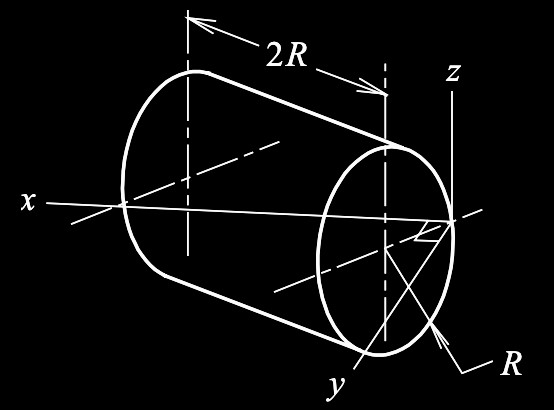
\includegraphics[scale=0.7,frame]{images/Q5_13.png}
% \end{figure}




\end{document}

